Der Aufbau des Projekts dreht sich rund um das Abspeichern, sowie die sinnvolle visuelle Darstellung von Daten. Dabei werden verschiedenste Programmiersprachen, Plattformen und Frameworks verwendet. \ref{fig:impl:FlexLoggerAufbau}

\begin{figure}
    \centering
    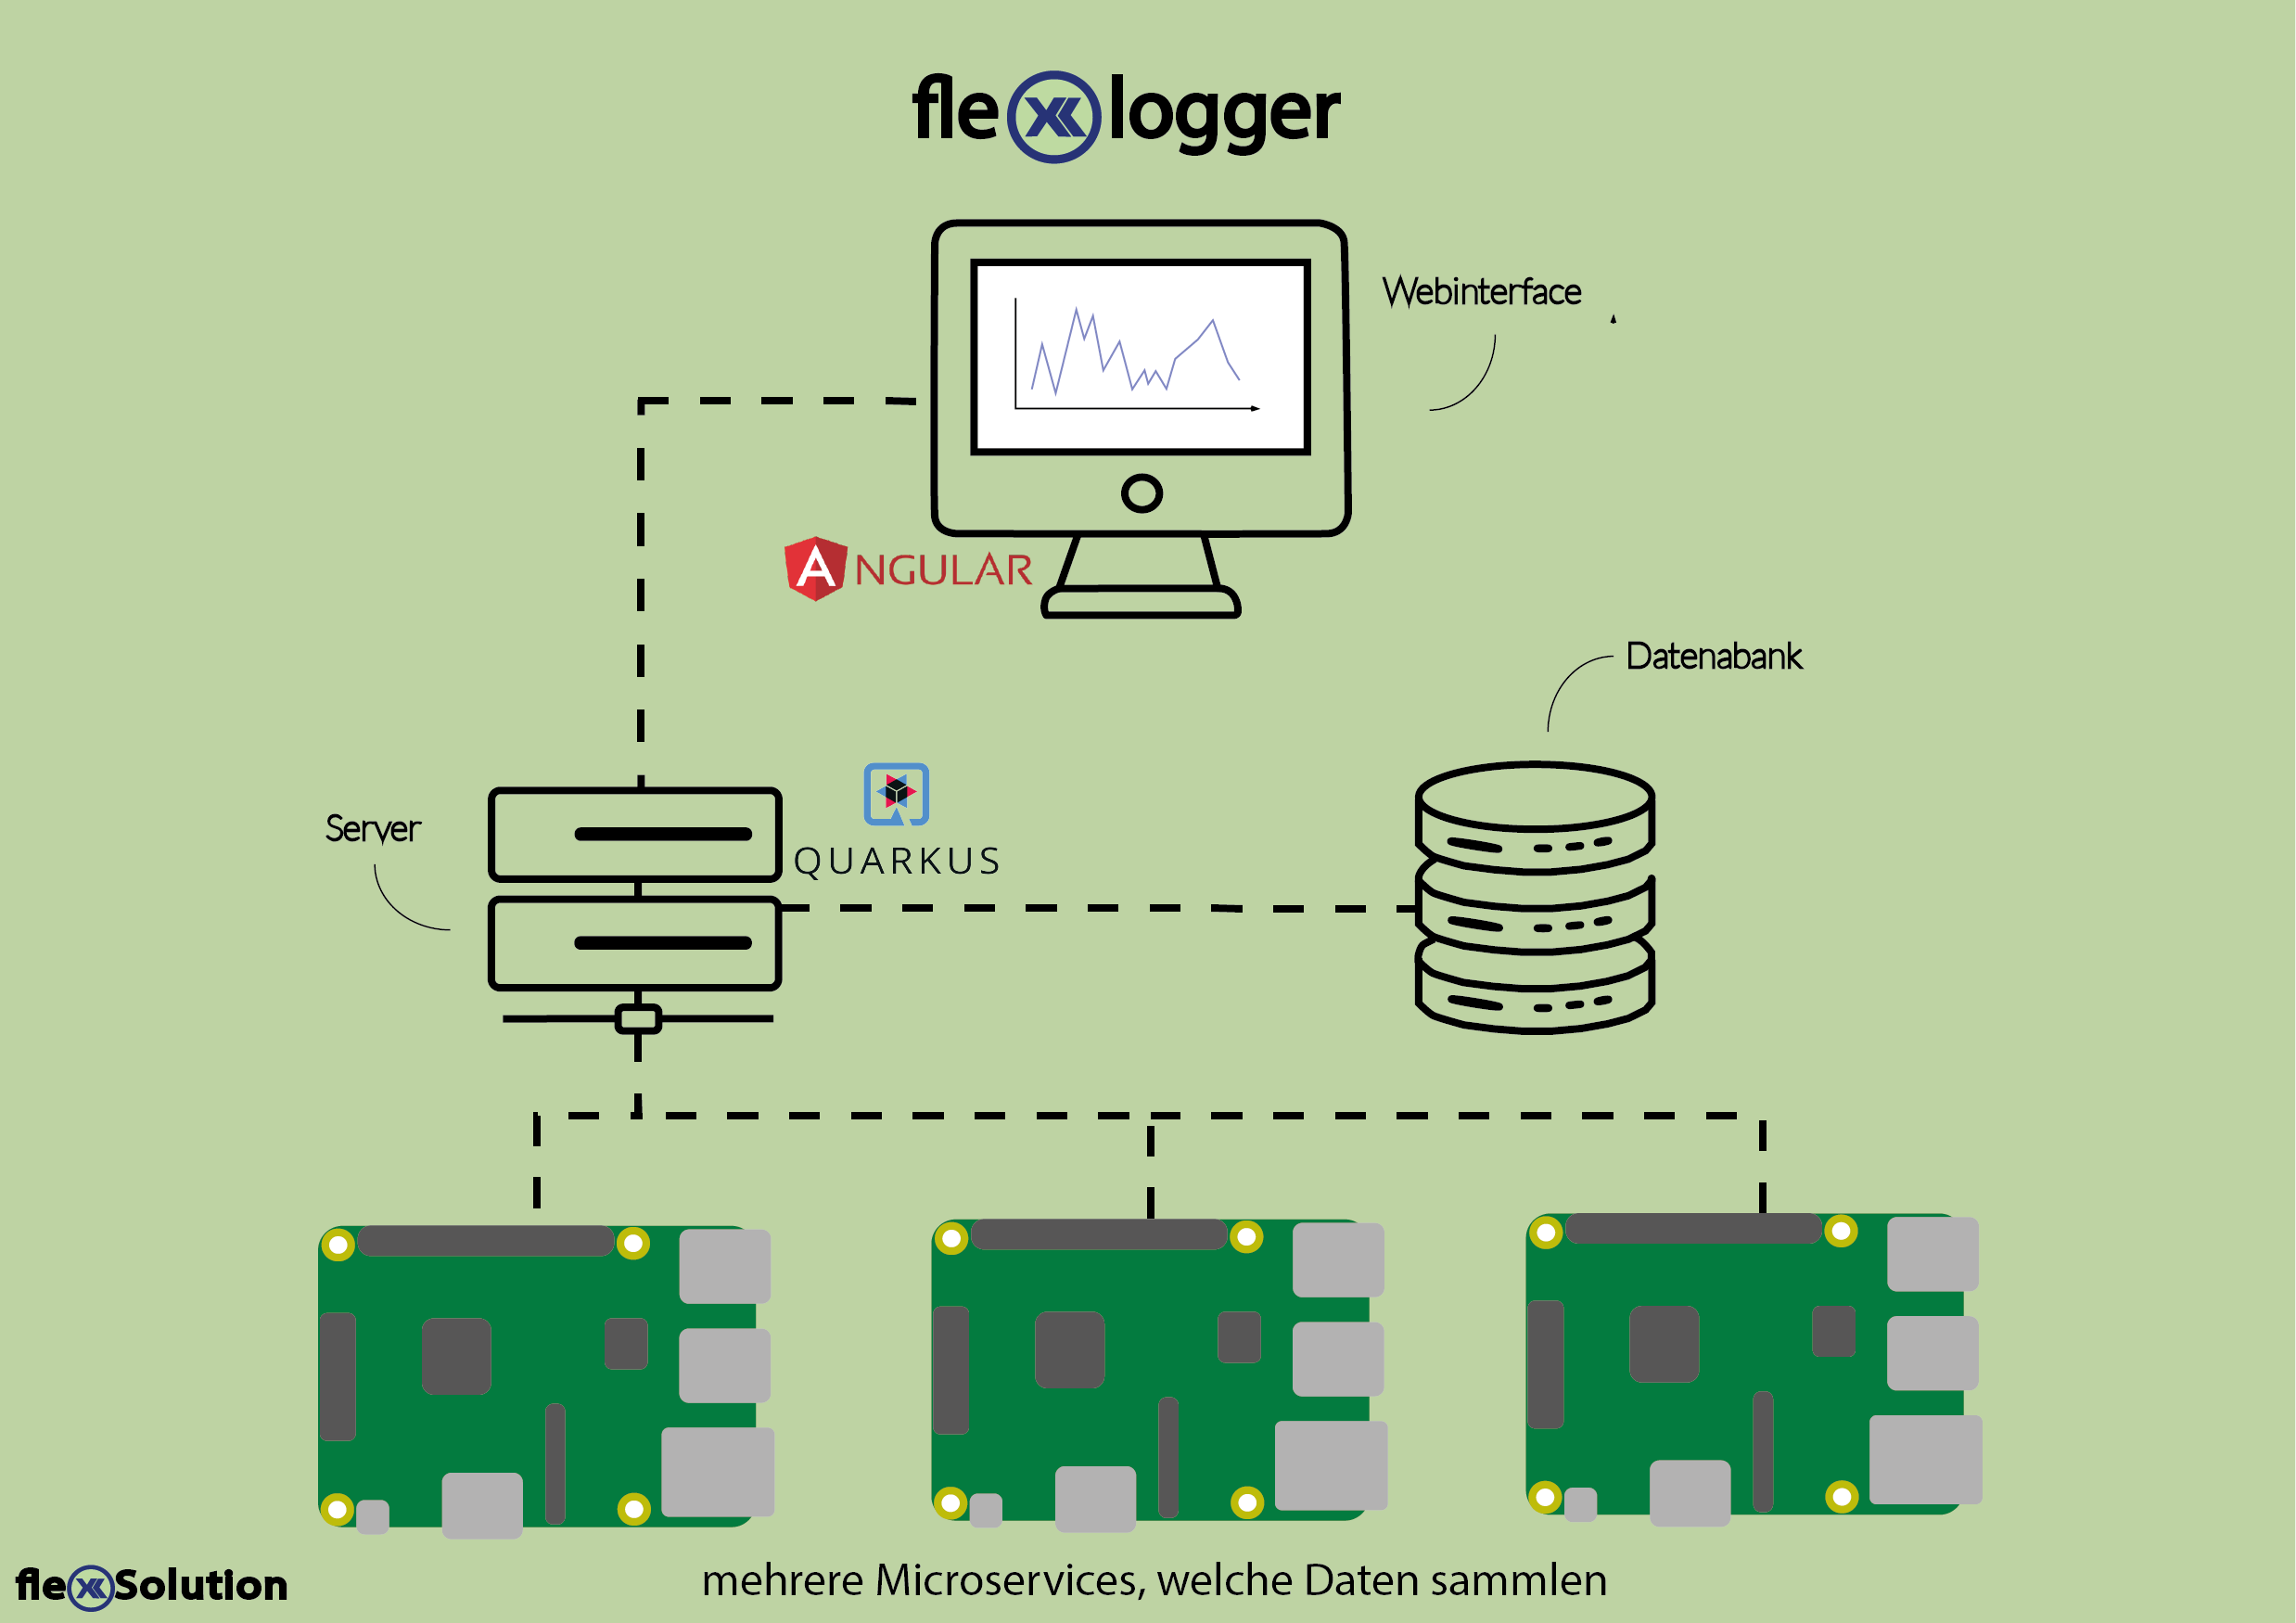
\includegraphics[scale=0.7]{pics/webinterface.png}
    \caption{Aufbau des Flexloggers visuell dargestellt}
    \label{fig:impl:FlexLoggerAufbau}
\end{figure}

\subsection{Beschreibung der Funktionen}
Die Funktionen des Projekts beziehen sich großteils auf 
\begin{compactitem}
    \item das Auslesen von Daten aus Datenpunkten mithilfe von Threads
    \item das Abspeichern von Daten in einer Datenbank durch Threads
    \item das spätere Auslesen der Daten aus der Datenbank, um diese sinnhaft visuell darstellen zu können
    \item die Verwendung von Formularen um (ausgewählte) Daten, in einem bestimmten Zeitpunkt graphisch in einem Diagramm darzustellen, oder eine CSV-Datei aus den Daten erstellen zu können
\end{compactitem}


\subsection{Logger}
Das sogenannte FS-Logger-Programm setzt sich aus mehreren Klassen zusammen, wie etwa einem DataJDBCAdapter und einer Hauptklasse namens FlexTaskFsLogger. Weiteres befindet sich in dem Programm eine Modelklasse namens LogEntry, welche die Attribute der eingetragenen LogEntries definiert. Um einen reibungslosen Ablauf zu garantieren, wird eine Blocking-Queue verwendet, welche Multithreading unterstützt. Das ganze Programm baut auf dem Producer-Consumer-Pattern auf.          
 
\subsubsection{DataJDBCAdapter}
Der DataJDBCAdapter ist dafür verantwortlich, eine Verbindung zu der PostgreSQL-Datenbank aufzubauen und somit die benötigten Objekte in einer Datenbank abzuspeichern (insert). Um diese Verbindung herzustellen, verwendet der JDBCAdapter eine URL, welche in einem String abgespeichert ist sowie einen Benutzernamen und ein Passwort. Innerhalb der connect-Methode werden diese Daten verwendet, sie gibt ein Connection-Objekt zurück, welches angibt, ob die Verbindung zur Datenbank erfolgreich war. Die connect-Methode wird innerhalb der darunterliegenden insertLogEntry-Methode aufgerufen. Wenn die Anbindung erfolgreich war, wird ein PreparedStatement mithilfe des vorher übergebenen SQL-String erstellt und darauffolgend ausgeführt. Somit wird erfolgreich ein neuer Datenbankeintrag in der Datenbank gespeichert. Falls während des ganzen Ablaufes ein unerwarteter Fehler auftauchen sollte, wird dieser mittels einer Java-Exception in die Konsole geschrieben.
 
\subsubsection{Main Klasse FlexTaskFsLogger}
Die Klasse FlexTaskFsLogger ist die Main-Klasse des Programms. Sie führt das Programm aus. Dieser Klasse werden auch folgende Methoden vererbt, da sie eine Subklasse der Klasse FlexTask ist:
\begin{compactitem}
    \item getNeededTaskParameters
    \item getNeededDeviceParameters
    \item isSingleDeviceTask
    \item closing
    \item initTask
\end{compactitem}
 
Zusätzlich befindet sich noch in der Klasse eine Getter- und Setter-Methode, diese sind allerdings lediglich für eine Zählvariable zuständig, um bestimmte Daten weniger oft in die Datenbank einzuspeichern. 
Die Hauptmethode des FlexTaskFsLogger ist die initTask-Methode. In ihr wird eine BlockingQueue mit dem generic Type LogEntry erstellt. Mithilfe dieser Blocking-Queue werden darauffolgend ein Producer und ein Consumer erstellt, welche die Blocking-Queue als Parameter übergeben bekommen. Nachfolgend werden jeweils zwei Producer-Threads und zwei Consumer-Threads erstellt und gestartet. Um eine zeitliche Einteilung zu haben, wird ein sogenannter TimerTask erstellt \ref{lst:impl:timerTask}, welcher wiederum auch ein neuer, unabhängiger Thread ist. Er wird dazu genutzt, um in einem gewissen Intervall Methoden oder Code-Blöcke aufzurufen. In diesem Fall wird der Task dazu verwendet, über den DataJDBCAdapter einen neuen Eintrag in der Datenbank zu speichern. Dazu wird zuallererst überprüft, ob eine Variable, welche für das Starten und Stoppen des Tasks zuständig ist, auf true gesetzt wurde. Anschließend wird ein sogenannter StringBuilder, welcher aus einer Kette von Strings besteht, aus dem vorher erstellten Consumer geholt. Dieser StringBuilder besteht aus einem aneinandergeketteten Insert-Statement. Um die Ausführbarkeit des Stringbuilders zu gewährleisten, muss die letzte Stelle (an welcher sich ein Beistrich befindet) gelöscht werden und durch einen Strichpunkt ersetzt werden. \ref{lst:impl:timerTask}


\begin{lstlisting}[language=java,caption=TimerTask,label=lst:impl:timerTask]
    TimerTask timerTask = new TimerTask() {
        @Override
        public void run() {
            counter = true;
            if (producer.getRun()) {
                StringBuilder stringBuilder = consumer.getStringBuilder();
                stringBuilder.deleteCharAt(stringBuilder.length() - 1);
                stringBuilder.append(";");
                try {
                    dba.insertLogEntry(stringBuilder.toString());
                    // System.out.println("successful writing to db");
                } catch (Exception e) {
                    System.out.println(e);
                }

                stringBuilder.delete(0, stringBuilder.length());
                consumer.setStringBuilder(stringBuilder.append("INSERT INTO flexlogger(dp_name, value, unit, timestamp) VALUES "));
            }
        }
    }; 
\end{lstlisting}

Um das korrekt erstellte SQL-Statement nun ausführen zu können, wird in einem try and catch Statement die insertLogEntry-Methode des DataJDBCAdapters ausgeführt. Dabei wird der StringBuilder mit dem SQL-Statement, welches mithilfe der toString-Methode in einen String umgewandelt wird, übergeben.
 
Anschließend wird der eben verwendete StringBuilder geleert, indem die delete-Methode aufgerufen wird. Um einen neuen Insert-Aufruf zu ermöglichen, wird ein insert-Header über die setStringBuilder-Methode aus dem Consumer gesetzt.
 
Nun wird der vorher beschriebene TimerTask in einem eine Zeile davor erstellten Timer als Parameter übergeben.
 
Der nächste Abschnitt sorgt dafür, dass das Programm, also der Consumer und der Producer aus- und eingeschaltet werden kann. Dazu werden zuerst zwei Datenpunkte initialisiert. Diese werden durch das Setzen einer spezifischen Adresse und den Namen eines Datenpunkts erstellt. Dabei ist der Datenpunkt \texttt{logger\_nav\_status\_icon\_Click} dazu verantwortlich, darauf zu hören, ob sich ein Wert, welcher in diesem Datenpunkt gespeichert ist, geändert hat. Das heißt, wenn auf der eigens dafür erstellten Website der Ein- und Ausschaltknopf gedrückt wird, wird der Timer pausiert und das Programm schreibt keine Werte mehr in die Datenbank. Im Gegensatz dazu ist der \texttt{logger\_nav\_status\_icon\_State} dafür da, einen Wert für die Website zu übergeben. Damit wird die Farbe des Icons verändert, um dem User ein Feedback zu seiner Aktion zu geben.
Nachdem die Methode setDatapointChangedCommand mit dem \texttt{logger\_nav\_status\_icon\_Click} verbunden wird, wird aktiv auf den Datenpunkt gehört. Ein neuer DatapointCommand wird dabei übergeben, in ihm wird die execute-Methode überschrieben. In dieser Methode wird zuallererst eine temporäre Variable erhöht, sie ist dafür da, jeden zweiten Dateneintrag zu überspringen, da die HMI jedes Mal zwei Werte schickt, allerdings nur einer benötigt wird. In Folge darauf wird in einem If-Statement der Wert des \texttt{logger\_nav\_status\_icon\_State} Datenpunkts geändert, um die Farbe des Einschalt Icons zu verändern. Zusätzlich wird die startOrStop Variable auf false gesetzt und der Producer und der Consumer werden mithilfe der Übergabe von ‚false‘ in der setRun-Methode gestoppt. Im else-Zweig des If-Statements wird genau das Gegenteilige bewirkt, das bedeutet Producer und Consumer werden gestartet und die \texttt{logger\_nav\_status\_icon\_State} wird wieder auf den ursprünglichen Wert geändert.
 
\subsubsection{LogEntry Klasse}
Dies ist die Model-Klasse des Programms. In ihr werden die Attribute des LogEntries festgelegt. Diese beinhalten die dp-id, das bedeutet die Id des Datenpunktes, welcher gespeichert werden soll. Außerdem wird der Wert des Datenpunktes, die Einheit und der Timestamp, also der genaue Zeitpunkt, an welchem der LogEntry erstellt wurde, angelegt. In der Klasse befinden sich zusätzlich Getter und Setter für die Attribute und ein Konstruktor.
 
\subsubsection{Blocking Queue - Producer }
Diese Klasse ist der Producer der Blocking Queue, soll heißen in dieser Klasse werden die Objekte in die Blocking Queue hinzugefügt.
 
Es lassen sich zwei Attribute im Producer finden, die Blocking Queue, in welche die Objekte später hinzugefügt werden und eine Boolean Variable, welche den Namen "run" trägt. Sie ist dafür verantwortlich, den Producer zu deaktivieren bzw. zu aktivieren. Unterhalb der Attribute befinden sich ein Konstruktor, um die Blocking-Queue zu übergeben und ein Getter und ein Setter für die run-Variable.

Die Hauptmethode der Klasse ist die run-Methode. Hier wird ein neuer DatapointCommand erstellt, in welchem die execute-Methode überschrieben wird. Innerhalb der execute-Methode wird ganz oben eine Counter Variable initialisiert, sie ist dafür verantwortlich, bestimmte Daten von Datenpunkten nur jedes zweite Mal in die Blocking Queue hinzuzufügen. Danach befindet sich ein if-Statement, welches überprüft, ob der Code im Consumer ausgeführt werden soll oder nicht. In diesem if-Statement befindet sich ein Switch für den specificDataType, welcher je nach DataType einen bestimmten Codeteil ausführt. In dem einen Codeteil wird die counter-Variable auf true oder false überprüft (bei einem false wird der Datenteil nicht in die Blocking-Queue hinzugefügt), in dem anderen wird dies ignoriert.
 
Allerdings kümmern sich beide Codeteile darum, die jeweiligen Daten als LogEntry zu erstellen und diesen anschließend in die Blocking Queue zu pushen. \ref{lst:impl:logEntryBlockingQueue}

\begin{lstlisting}[language=java,caption=LogEntry in BlockingQueue hinzufügen,label=lst:impl:logEntryBlockingQueue]
    try {
            LogEntry logEntry = new LogEntry(datapointResult.getDpId(), datapointResult.getValue(), "A", datapointResult.getTimestamp());
            blockingQueue.put(logEntry);
        } catch (InterruptedException e) {
            throw new RuntimeException(e);
        }
\end{lstlisting}

 
Mithilfe des Codes, welcher sich unterhalb des erstellten DataPointCommands befindet, wird über die Datenpunkte des jeweiligen Geräts iteriert und anschließend wird der oben liegende Codeteil bei einer Änderung ausgeführt. \ref{lst:impl:datenpunkteIterieren}
 
\begin{lstlisting}[language=java,caption=Datenpunkte des jeweiligen Geräts iterieren,label=lst:impl:datenpunkteIterieren]
    for (Device dev : StaticData.devices.getDevices()) {
        for (Datapoint dp : StaticData.datapoints.getDatapoints(dev.getId())) {
            if (!dp.getSpecificDataType().isEmpty()) {
                dp.setDatapointChangedCommand(dpCmd);
            }
        }
}
\end{lstlisting}

\subsubsection{Blocking Queue - Consumer }
In dieser Klasse geht es um den Consumer der Blocking Queue, das bedeutet vom Consumer werden Objekte aus der Blocking Queue genommen und diese weiterverarbeitet. Die Attribute in dieser Klasse sind so wie in der Producer Klasse eine Blocking-Queue, sowie die run-Variable, um den Consumer zu aktivieren bzw. zu deaktivieren. Im Konstruktor wird wiederum die Blocking-Queue übergeben.
 
In der run-Methode der Klasse wird in einem while-True ein if-Statement ausgeführt, in welchem sich ein Try-and-Catch-Statement befindet. In diesem wird das benötigte Objekt aus der Blocking-Queue geholt und anschließend in einen StringBuilder als gültiges SQL-Statement hinzugefügt. \ref{lst:impl:logEntryBlockingQueueConsumer}

 \begin{lstlisting}[language=java,caption=Daten aus BlockingQueue herausnehmen,label=lst:impl:logEntryBlockingQueueConsumer]
    try {
        LogEntry logEntry = this.blockingQueue.take();
        stringBuilder.append("('" + logEntry.getDpId() + "'," + logEntry.getValue() + "," + "'A'," + logEntry.getTimeStamp() + "),");
    } catch (InterruptedException e) {
        e.printStackTrace();
    }
\end{lstlisting}

Unterhalb befindet sich noch eine Getter- und Setter-Methode für den StringBuilder sowie die run-Variable.
 
\subsection{Quarkus Backend}
Das Backend setzt sich zusammen aus der Programmiersprache Java und dem Java-Framework Quarkus.
 
\subsubsection{LogEntry Klasse}
Hier werden die Attribute des LogEntries festgelegt. Diese beinhalten wie auch im Programm FlexTaskFsLogger die dp-id, den Wert, die Einheit und einen aktuellen Timestamp des Eintrags.
Auch beinhaltet ist ein Konstruktor, Getter- und Setter-Methoden für die Attribute sowie eine toString-Methode, um die Attribute formatiert zurückgeben zu können.
 
\subsubsection{LogEntry Ressource}
Mithilfe dieser Klasse werden bestimmte Daten an bestimmte vorher definierte Adressen geschickt.
Der vorher definierte Path ‚/logEntry‘ wird dabei bei jeder Anfrage am Anfang der Adresse verwendet.
Um das davor erstellte LogEntry-Repository zu verwenden, wird es am Anfang der Methode mit dem Schlüsselwort new initialisiert.
 
In der Ressource befinden sich verschiedenste GET-Methoden, welche alle einen anderen Nutzen haben:
 
\begin{compactitem}
    \item getAll(): Hier wird durch die Übergabe der Parameter definiert, in welchem Zeitraum die benötigten Daten zurückgegeben werden. Diese Parameter werden mithilfe von PathParam übergeben, soll heißen die Daten werden über die URL übergeben. Zusätzlich steht über der Methode ein \texttt{@Produces(MediaType.APPLICATION\_JSON)}, um festzulegen, in welchem Format der Rückgabewert zurückgegeben wird. In diesem Fall ist es das JSON-Format.
    \item getByName(): Diese Methode ist sehr ähnlich zur getAll()-Methode. Lediglich wird ein zusätzlicher Name übergeben und somit die getByName-Methode des Repositories verwendet.
    \item getCSV(): In dieser Methode wird im Pfad neben den Daten ein FilePath angegeben, in welchem die CSV-Datei gespeichert werden soll. Mithilfe der getCSVAll-Methode aus dem Repository wird die CSV-Datei anschließend im richtigen Pfad gespeichert.
    \item getCSVByName(): Die Methode hat eine ähnliche Funktion wie die getCSV()-Methode. Der entscheidende Punkt dabei ist, dass ein Name übergeben werden kann, welcher die Rückgabedaten beeinflusst, da so nur die Daten mit dem richtigen Namen als CSV-Datei erstellt wird. 
    \item insert(): Mithilfe dieser Methode kann ein neuer LogEntry in die Datenbank eingefügt werden. Als Parameter in der insertLogEntry-Methode des Repositories wird dabei ein neu erstellter LogEntry übergeben.
    \item downloadFile(): Um das vorher erstellte CSV-File zu downloaden, wird diese Methode genutzt. In diesem Fall ist der Rückgabewert der Methode mit einem \texttt{@Produces(\{"text/csv"\})}definiert, da es sich dabei um eine CSV-Datei handelt. Zuallererst wird in der Methode ein File-Name, ein Pfad, sowie ein File erstellt. Der Pfad und der File-Name ist dabei jeweils vom Datentyp String, das File ist vom Datentyp File und wird mithilfe des Pfads als Parameter erstellt. Um zu überprüfen, dass der Pfad existiert, wird mithilfe eines IF-Statements die Methode exists() beim vorher erstellten File als Überprüfung herangezogen. Wenn dieses IF-Statement feststellt, dass das File nicht existiert, wird eine RuntimeException geworfen. Diese enthält die Nachricht "File not found: " und den zugehörigen File-Namen. Bei einem erfolgreichen Erstellen des Files wird ein ResponseBuilder namens res erstellt. Dieser enthält die Response OK sowie das File. Zusätzlich wird bei dem ResponseBuilder ein Header gesetzt, in welchem sich unter anderem der FileName befindet. Schlussendlich wird der ResponseBuilder mit einem Build-Statement zurückgegeben. Somit wurde das vorher erstellte File erfolgreich heruntergeladen und kann nun mithilfe von einem passenden Programm geöffnet und gesichtet werden.
\end{compactitem}
 
\subsubsection{LogEntry Repository}
Das Repository des Backends ist dafür verantwortlich, eine Verbindung zur Datenbank herzustellen und die richtigen Daten an die Ressource weiterzugeben. Zuallererst werden drei verschiedene Strings definiert, um Zugriff auf die Datenbank zu erlangen. Der erste ist dabei die URL, um sich zur Postgres-Datenbank zu verbinden. Der zweite und dritte String definiert den User sowie das Passwort, um Zugriff zur Datenbank zu erlangen.
 
Die erste Methode in der Klasse trägt den Namen connect. Wie der Name schon sagt, wird in der Methode mithilfe eines DriverManagers eine Verbindung auf die Datenbank aufgebaut und zurückgegeben, welche in den folgenden Methoden verwendet werden kann.
 
\begin{lstlisting}[language=java,caption=Connect to SQL Database,label=lst:impl:connect]
    /**
    * Connect to the PostgreSQL database
    *
    * @return a Connection object
    */
   public Connection connect() throws SQLException {
       return DriverManager.getConnection(url, user, password);
   }  
\end{lstlisting}
 
Jede der nachfolgenden Methoden ist für eine bestimmte Aktion auf der Datenbank zuständig.
Um alle vorhandenen LogEntries in einem bestimmten Datumsbereich zu erlangen, kann die getAll-Methode verwendet werden. Die übergebenen Parameter sind dabei das Anfangs- und das Enddatum, sowie die Anfangs- und die Endzeit. Anfangs wird nun ein Set von LogEntries erstellt, in welchem nachfolgend die Daten hinzugefügt werden. Um das Datum und die Zeit in Millisekunden umwandeln zu können, da nur diese später in einem SQL-Statement verwendet werden können, wird eine convertToMillis-Methode verwendet. So wird eine Start- und Endzeit in Millisekunden erstellt.
Um die Daten, welche zwischen dem Start- und dem Enddatum liegen, zu bekommen, wird in einem SQL-Statement definiert, dass der Timestamp des jeweiligen LogEntries größer als die Startmillisekunden, und kleiner als die Endmillisekunden ist. Außerdem werden die Daten nach dem timestamp geordnet. Anschließend wird eine Verbindung zur Datenbank aufgebaut. Um das vorher erstellte SQL-Statement nutzen zu können, wird ein PreparedStatement genutzt. In diesem werden die beiden Parameter startMillis und endMillis gesetzt. Aus diesem PreparedStatement wird nun ein ResultSet gewonnen, durch die Methode executeQuery. Um vollständige LogEntries zu erhalten, werden alle ResultSets mithilfe einer while-Schleife durchgegangen. Jeder der LogEntries wird zu dem Set namens LogEntries hinzugefügt. Um die richtigen Spalten der LogEntries zu bekommen, wird der Name der Spalte verwendet.
 
Bei einem Fehler in der Verbindung zur Datenbank wird eine Fehlermeldung ausgegeben. Bei einem Erfolg wird das Set von LogEntries zurückgegeben und kann somit in der Ressource verwendet werden.
 
Die getByName-Methode ist sehr ähnlich zur getAll-Methode. Der einzige Unterschied ist, dass als Parameter zusätzlich ein Name mitübergeben wird. Dieser wird zusätzlich im SQL-Statement gesetzt und somit werden alle LogEntries, welche einen anderen Namen tragen, aussortiert. Zurückgegeben wird erneut ein Set aus LogEntries.
 
Die bereits verwendete convertToMillis-Methode befindet sich direkt unter der vorigen Methode. In ihr wird das Datum und die Zeit als gemeinsamer String erstellt. Dieser String wird nun verwendet, um eine Variable des Typs LocalDateTime zu erstellen. Dieses wird nach dem richtigen Formatieren bzw. Umwandeln zurückgegeben.
 
Der nächste Abschnitt des Repositories ist für alle Methoden rund um das Erstellen von CSV-Dateien zuständig. Die ersten beiden Methoden unterteilen jeweils, ob ein Name mitübergeben wurde, oder nicht. Die Parameter sind dabei das Anfangs- und Enddatum, sowie die Anfangs- und Endzeit. Bei der zweiten Methode wird nun ein Name zusätzlich übergeben. Der meiste Teil der Methoden ist relativ ähnlich, zuerst wird ein Set von LogEntries erstellt. Je nach Methode werden mithilfe der Parameter die richtigen LogEntries mit der getByName-Methode bzw. der getAll-Methode in dem Set gespeichert. Nachfolgend wird aus dem Set ein Stream erstellt, dabei wird jedes logEntry-Objekt zu einem String umgewandelt. Anschließend wird jeweils die Methode writeToCSVFile aufgerufen, welche sich direkt unter den anderen zwei Methoden befindet. Übergeben wird dabei beide Male der zuvor erstellte Stream mit den Strings, sowie ein neu erstelltes File mit einem vorher erstellen FilePath. \ref{lst:impl:logEntryZuCSV}

\begin{lstlisting}[language=java,caption=LogEntrySet zu CSV umwandeln,label=lst:impl:logEntryZuCSV]
    Set<LogEntry> logEntrySet = getAll(startDate, startTime, endDate, endTime);
    Stream<String> stringSet = logEntrySet.stream().map(logEntry -> logEntry.toString());
    writeToCsvFile(stringSet, new File(filePath));
\end{lstlisting}

Die erste Zeile in der writeToCSVFile-Methode \ref{lst:impl:downloadCSV} konvertiert das eben übergebene Set zu einer Liste. In diesem Prozess wird eine weitere Methode angewendet, welche den Namen convertToCSVFormat trägt. Mithilfe eines Map-Befehls wird die Methode auf jeder Zeile des Sets angewendet. Die convertToCSVFormat-Methode gibt dabei die übergebene Zeile als Stream zurück, wobei zwischen den einzelnen Werten in einer Zeile ein Semikolon eingefügt wird. Als nächstes wird ein BufferedWriter verwendet. Dieser wird als neue Instanz erstellt, mit dem Übergabeparameter eines neuen FileWriters, in welchem das am Kopf der Methode übergebene File übergeben wird. Der BufferedWriter ist von einem Try-and-Catch umgeben. Dies ist erforderlich, um bei einem eventuell auftretenden Fehler, wie etwa einem falschen Filepath oder fehlenden Berechtigungen, mit einer Fehlermeldung richtig reagieren zu können. In diesem Try-and-Catch wird nun jede Zeile der vorher erstellten Liste mithilfe einer For-Schleife durchgegangen. Mit den Methoden write() und newLine() wird somit die CSV-Datei Zeile für Zeile erstellt.

\begin{lstlisting}[language=java,caption=CSV-File herunterladen,label=lst:impl:downloadCSV]
    List<String> collect = logEntrySet
                .map(this::convertToCsvFormat)
                .collect(Collectors.toList());
        
    try (BufferedWriter bw = new BufferedWriter(new FileWriter(file))) {
        for (String line : collect) {
            bw.write(line);
            bw.newLine();
        }
    }   catch (Exception e){
        e.printStackTrace();
    }
\end{lstlisting}

Die letzte Methode im Repository ist die insertLogEntry-Methode. Wie der Name bereits verrät, ist sie dafür zuständig, neue LogEntries in der Datenbank zu speichern. Um einen neuen LogEntry zu speichern, wird zuallererst ein String erstellt, welcher ein Insert-Statement enthält.
Danach wird eine Verbindung zur Datenbank mithilfe der connect-Methode hergestellt. Durch ein PreparedStatement, welches aus einem SQL-String geformt wird, können alle Parameter gesetzt werden. Diese beinhalten die dpId (der Name des Datenpunkts), die value (den Wert des Datenpunkts), die unit (die Einheit des Datenpunkts), sowie den timestamp (wann der Datenpunkt erstellt wurde). Nachdem alle Parameter gesetzt wurden, wird ein executeUpdate durchgeführt, mithilfe dessen der neue LogEntry in die Datenbank geschrieben wird.
 
\subsection{Angular Frontend}
%% sehr einfache Beschreibung der Website mit vielen Screenshots von den einzelnen Komponenten (Button/ Eingabefeld / was wird wann angezeigt etc.)
Die Website des Projekts wurde mithilfe von Angular umgesetzt. Die Hauptfunktion liegt dabei bei dem Anzeigen von Diagrammen mit den jeweiligen ausgewählten Daten, sowie dem Generieren einer CSV-Datei.
 
 
\subsubsection{Website - User/Anwender Ansicht}
Die erste Seite, welche zu sehen ist, ist die Hauptseite \ref{fig:impl:FlexLoggerHauptseitenAnsicht}. Auf ihr ist zuerst ein großes Bild zu finden, gleich darunter kann die Schrift "Lassen Sie sich ihre gewünschten Diagramme anzeigen" erkannt werden.
Durch drei verschiedene Formulare, welche sich direkt unter der großen Überschrift befinden, können verschiedenste Funktionen genutzt werden. Jedes dieser Formulare besitzt dabei einen anderen Zweck.
 
\begin{compactitem}
    \item Formular 'Alle Diagramme': Das erste ist dafür zuständig, alle Diagramme in einem bestimmten Zeitraum anzuzeigen. Wenn der Button \ref{fig:impl:FlexLoggerHauptseitenAnsichtButton} dieses Formulars betätigt wird, erfolgt eine Weiterleitung auf eine weitere Seite. Auf dieser kann nun zwischen allen Diagrammen mithilfe von automatisch generierten Buttons wechseln \ref{fig:impl:FlexLoggerDiagrammAnsicht}.
    \item Formular 'Diagramm per Name': Das zweite Formular hat eine ähnliche Funktion. Lediglich kann hier das Diagramm, welches angezeigt werden soll, im Formular mitübergeben werden. Durch den Button \ref{fig:impl:FlexLoggerHauptseitenAnsichtButton} erfolgt nun eine direkte Weiterleitung zum gewünschten Diagramm.
    \item Formular 'CSV File': Eine ganz andere Funktion hat das letzte Formular. In ihm wird zwar genauso der Wunschzeitraum angegeben, allerdings wird nach Betätigen des Buttons \ref{fig:impl:FlexLoggerHauptseitenAnsichtButton} ein CSV-File generiert und anschließend heruntergeladen. In diesem werden alle Daten übersichtlich angezeigt. \ref{fig:impl:FlexLoggerHauptseitenAnsichtCSV}
\end{compactitem}
 
Die Formulare können dadurch genutzt werden, dass zuerst jeweils die richtigen Von-, Bis-Daten angegeben werden müssen. \ref{fig:impl:FlexLoggerHauptseitenAnsichtZeitraum} Wenn die Daten falsch eingegeben wurden (soll heißen es wurde ein Datum eingegeben, welches hinter dem Anfangsdatum liegt bzw. bei einem gleichen Anfangs- und Enddatum muss die Endzeit hinter der Anfangszeit liegen), wird eine Fehlermeldung ausgegeben, um den User auf seine fehlerhafte Eingabe aufmerksam zu machen. Bei dem Formular 'Diagramm per Name' muss zusätzlich ein Name angegeben werden, sonst wird erneut eine Fehlermeldung angezeigt. Wenn allerdings das Formular 'CSV-File' betrachtet wird, gibt es eine zusätzliche Fehlerüberprüfung, welche direkt nach dem Betätigen des Buttons ausgeführt wird. Werden keine Daten aus der Datenbank für den eingegebenen Zeitraum gefunden, wird eine passende Fehlermeldung angezeigt. \ref{fig:impl:FlexLoggerHauptseitenAnsichtFehlermeldung}
 
\begin{figure}
    \centering
    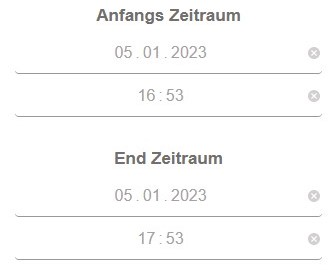
\includegraphics[scale=1]{pics/FlexLoggerWebsiteFormulare_zeitraum.jpg}
    \caption{Formular Zeitraum}
    \label{fig:impl:FlexLoggerHauptseitenAnsichtZeitraum}
\end{figure}
 
\begin{figure}
    \centering
    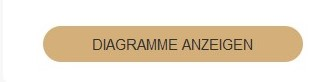
\includegraphics[scale=1]{pics/FlexLoggerWebsiteFormulare_button.jpg}
    \caption{Formular Button}
    \label{fig:impl:FlexLoggerHauptseitenAnsichtButton}
\end{figure}
 
\begin{figure}
    \centering
    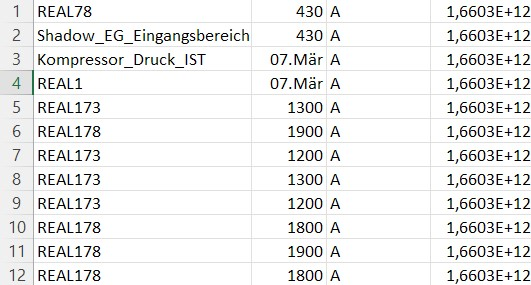
\includegraphics[scale=1]{pics/csv_datei_beispiel.jpg}
    \caption{CSV-Datei Beispiel Ausgabe}
    \label{fig:impl:FlexLoggerHauptseitenAnsichtCSV}
\end{figure}
 
\begin{figure}
    \centering
    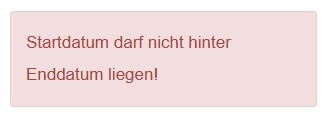
\includegraphics[scale=1]{pics/FlexLoggerWebsite_Fehlermeldung.jpg}
    \caption{Webseite Fehlermeldung}
    \label{fig:impl:FlexLoggerHauptseitenAnsichtFehlermeldung}
\end{figure}
 
 
\begin{figure}
    \centering
    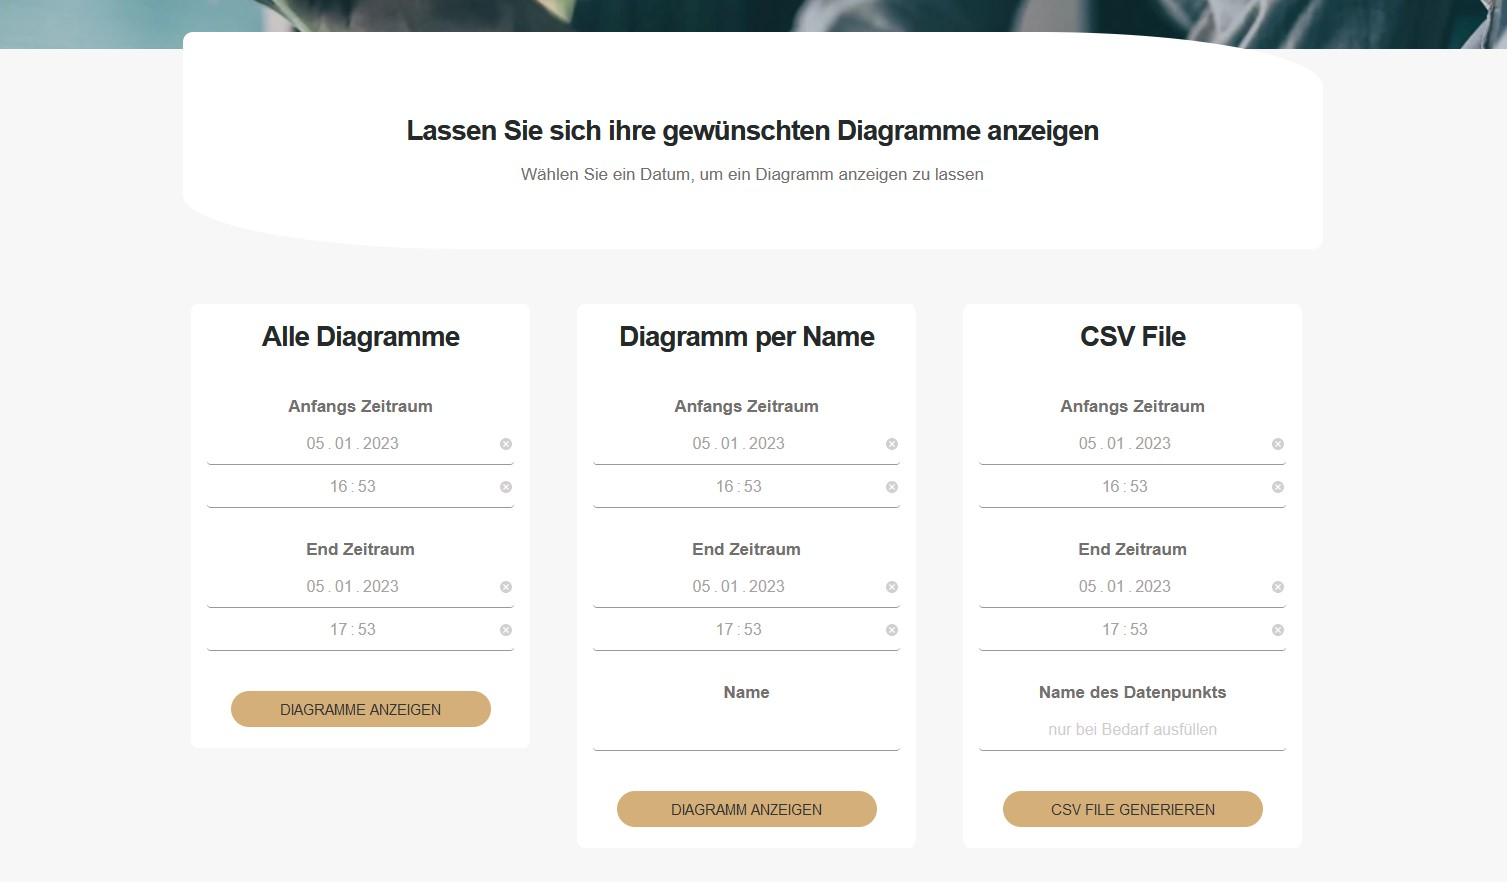
\includegraphics[scale=0.45]{pics/FlexLoggerWebsiteFormulare.jpg}
    \caption{Website Hauptseitenansicht}
    \label{fig:impl:FlexLoggerHauptseitenAnsicht}
\end{figure}
 
\begin{figure}
    \centering
    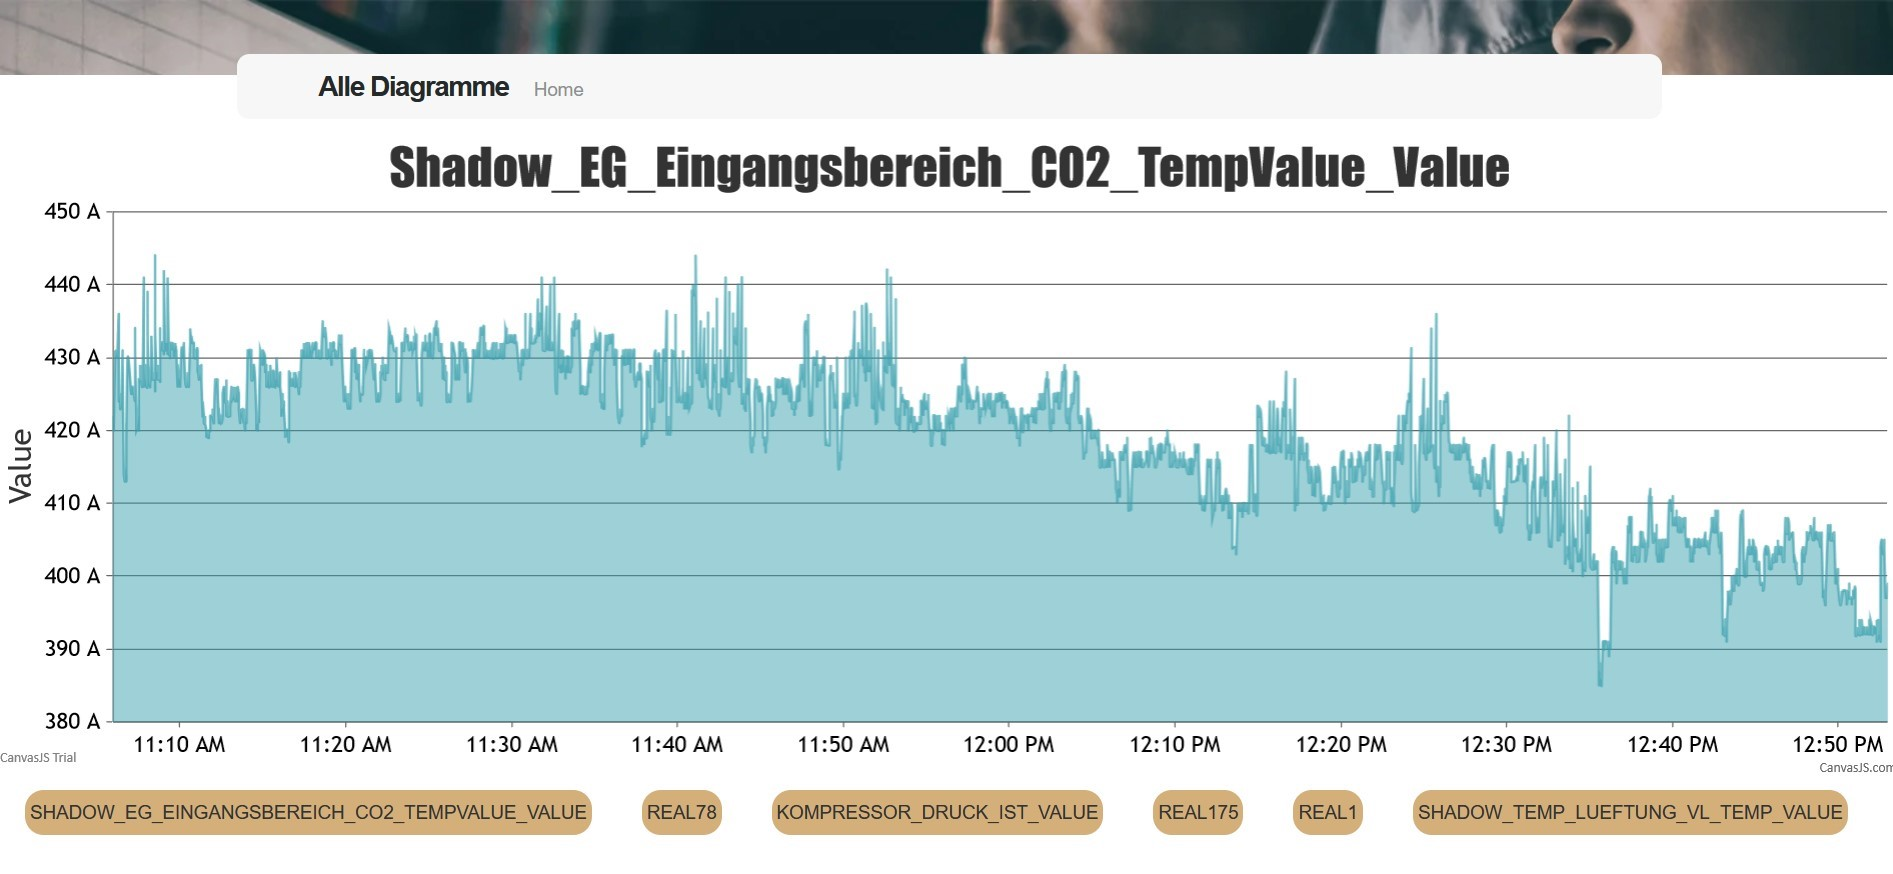
\includegraphics[scale=0.35]{pics/FlexLoggerWebsiteDiagramm.jpg}
    \caption{Website Diagrammansicht}
    \label{fig:impl:FlexLoggerDiagrammAnsicht}
\end{figure}
 
\subsubsection{App-Component}
In der TypeScript Klasse der App-Komponente wird selbst ein Titel definiert, dieser trägt in diesem Fall den Namen „flexloggerFE2". Im HTML-File ist dabei ein Router-Outlet definiert. Durch dieses wird das Routing im Projekt ermöglicht. Das heißt, jede Komponente wird praktisch in der App-Komponente angezeigt. In der app-routing-module Klasse werden alle Pfade des Projekts definiert. Dabei wird jeweils ein String als Pfad angegeben sowie eine Komponente definiert, zu welcher der Pfad führen soll. Zusätzlich wird bei den Modulen des Projekts ein RouterModule hinzugefügt, welches zusätzlich die Methode forRoot verwendet, in welchem die vorher definierten Routen als Parameter übergeben werden. In der App-Module-Klasse werden noch weitere Module hinzugefügt:
 
\begin{compactitem}
    \item BrowserModule: Stellt einen Service zur Verfügung, mit welchem eine Browser-App gestartet, sowie laufen gelassen werden kann.   
    \item AppRoutingModule: Ermöglicht das Navigieren zwischen verschiedenen Komponenten.    
    \item HttpClientModule: Mithilfe dieses Moduls können Netzwerk Requests abgesetzt werden. Diese inkludieren GET, POST, PUT, PATCH und DELETE.   
    \item FormsModule: Durch dieses Modul können template-driven Forms erstellt werden.   
    \item ReactiveFormsModule: Mithilfe dieses Moduls kann ein ReactiveForm verwendet werden.
\end{compactitem}
 
\subsubsection{Home-Component}
Die ist die Hauptkomponente des Programms. In ihr werden 3 Formulare definiert, jedes davon hat eine andere Funktion. Im Konstruktor der Komponente werden verschiedenste Parameter übergeben:
 
\begin{compactitem}
    \item HttpService: Dies ist der Service, mithilfe dessen eine Server-Verbindung zum Backend aufgebaut werden kann.   
    \item Router: Mithilfe dieses in Angular eingebauten Features kann auf der Website zwischen den Komponenten gewechselt werden.       
    \item ActivatedRoute: Mithilfe dieses Parameters können Daten über Komponenten hinweg übergeben werden.   
    \item FormBuilder: Durch diesen Parameter können reaktive Formulare erstellt werden
    \item ValidatorService: Wird später verwendet, um die Richtigkeit der Eingabe bei den Formularen zu garantieren.
\end{compactitem}
 
Im Konstruktor selbst, wird das heutige Datum sowie das heutige Datum plus einer Stunde gesetzt.
Um die Komponente zu initialisieren, wird in der ngOnInit()-Methode die initForms-Methode aufgerufen. Diese initialisiert alle 3 Formulare, indem sie die Variablen in den Formularen, sowie Validatoren setzt. Dabei wird bei den Variablen jeweils ein Standardwert gesetzt. Die gesetzten Validatoren überprüfen dabei, ob die Daten korrekte Eingaben in den Formularen sind.
 
Weiteres finden sich in der Komponente zwei Methoden, welche sich um das Routing kümmern. Diese kommen beim Klicken der Buttons der Formulare zum Einsatz, um die Komponente, welche angezeigt wird, zu wechseln. Die benötigten Daten werden dabei in der URL übergeben.
 
Die nachfolgende Methode ist für das Generieren sowie das Downloaden einer CSV-Datei zuständig. Zuallererst wird die checkCSV-Methode aufgerufen, in welcher überprüft wird, ob in dem ausgewählten Zeitraum Daten verfügbar sind.
 
Wenn die checkCSV-Variable als true gesetzt wurde, wird überprüft, ob der Namenparameter im Formular nicht leer ist. Trifft dies ein, wird mithilfe eines Timers und des Http-Service eine CSV-Datei generiert, welche alle Datenpunkte in dem richtigen Datumsbereich generiert. Nachdem das Generieren erfolgreich abgeschlossen wurde, wird der Download der Datei gestartet. Dieser Download wird mithilfe der window.open() Methode verwirklicht. Wenn der Namenparameter in dem Formular einen Namen enthält, so wird ein CSV-File generiert, welches nur die Daten eines Datenpunkts beinhält.
 
Wenn der Fall eintrifft, dass die checkCSV-Variable auf false gesetzt wurde, dann werden die Errors des Namenparameters auf true gesetzt. Dadurch wird unter dem Formular eine Fehlermeldung ausgegeben, um dem User eine Rückmeldung der Formulareingabe zu geben.
 
\subsubsection{Canvas-Chart-Component}
 
In dieser Komponente wird ein Diagramm erstellt, in welchem anschließend mithilfe von verschiedenen Buttons die gewünschten Daten angezeigt werden. 
 
Der erste wichtige Teil der Komponente ist das Erstellen der Diagrammoptionen. In diesen kann man verschiedenste Attribute eines Diagramms definieren:
 
\begin{compactitem}
    \item animationEnabled: Stellt ein, ob beim ersten Anzeigen eines Diagramms jeder Punkt des Diagramms flüssig geladen wird, um ein dynamischeres Ergebnis zu erhalten.   
    \item title: Setzt den Titel fest, welcher als Überschrift über dem Diagramm stehen soll.         
    \item axisY: Legt den Titel der Y-Achse fest, diese Einstellung kann genauso auf der X-Achse getätigt werden.   
    \item data: Dies ist die wichtigste Einstellung der Diagrammoptionen. Sie legt den Typ des Diagramms fest (in diesem Fall ist es ein Liniendiagramm), die Farbe des Diagramms und setzt die Datenpunkte fest. Beim ersten Laden der Seite werden die Datenpunkte der X- und Y- Achse auf 0 bzw. den 01.01.1970 gesetzt.
\end{compactitem}
 
Beim Laden der Seite wird zuerst im Konstruktor der Komponente eine Funktion namens onload() ausgeführt. Diese ist dafür zuständig, die erforderlichen Daten mithilfe des http-Service aus dem Backend zu bekommen. Zuerst werden hierfür die übergebenen Werte aus dem Formular mithilfe von Route-Snapshots übergeben. Anschließend wird durch den http-Service eine getLogEntries-Methode aufgerufen, diese gibt die Werte zurück, welche das erforderliche Datum besitzen. Diese werden nun in einem Array gespeichert, um weiter verwendet zu werden.
 
In der nächsten Zeile des Konstruktors befindet sich ein Timer, welcher nach 1 Sekunde den darauffolgenden Code durchführt. In diesem Code wird zuallererst eine getFiles-Methode ausgeführt, diese gibt das vorher erstellte Array zurück. Das IF-Statement eine Zeile darunter garantiert, dass die Länge des Arrays nicht 0 beträgt, ansonsten wird die Fehlermeldung "Zu Ihrem ausgewählten Zeitpunkt wurden keine Daten gefunden." ausgegeben. Bei einem positiven Ergebnis des IF-Statements werden nachfolgend vier Methoden aufgerufen:
 
\begin{compactitem}
    \item getListOfDatapointNames(): Diese Methode kümmert sich darum, eine Liste der Namen für die Buttons zu erstellen. Diese Buttons sind später dafür zuständig, zwischen den angezeigten Daten zu wechseln.
    Um zu verhindern, dass der Name eines Datenpunkts öfters in der Liste vorkommt, wird am Beginn eine Boolean-Variable namens nameInList erstellt. Diese wird vorerst auf False gesetzt.
    Anschließend wird ein vorher initialisiertes Array auf ein leeres Array gesetzt, in welches danach die Namen hinzugefügt werden. Um alle Namen aus den Daten zu erlangen, wird eine for-Schleife verwendet, welche alle vorher erhaltenen Daten durchgeht. Der erste Name wird immer hinzugefügt, daher wird, wenn die Länge des leeren Arrays 0 ist, der erste Name hinzugefügt. Sonst wird eine weitere for-Schleife betreten, welche alle Elemente der Liste der Namen durchgeht. Wenn ein Element bereits vorhanden ist, wird die nameInList Variable auf true gesetzt. Später wird in einem weiteren If-Statement überprüft, ob diese Variable auf True oder False gesetzt ist. Bei einem False wird dabei der Name in die Liste hinzugefügt. Durch dieses Verfahren wird sichergestellt, dass kein Name doppelt in der Liste vorkommt und somit Buttons nicht doppelt angezeigt werden.   
    \item changeData()
    Hier werden die geänderten Daten in den Diagrammoptionen gespeichert. Um dies umzusetzen, wird als Parameter ein String namens filterString übergeben. Mithilfe dessen und einer For-Schleife werden alle Datenpunkte herausgefiltert, welche nicht den gewünschten Namen besitzen. Die richtigen Daten werden nun im Array dynamicLogLines gespeichert. Nach dem Aussortieren der Daten wird mit einem IF-Statement überprüft, ob die erste Stelle des dynamicLogLines-Arrays nicht undefiniert ist. Wenn dies der Fall ist, werden der erste Datenpunkt, sowie der Titel in den Diagrammoptionen gesetzt. Danach werden die restlichen Datenpunkte mithilfe einer For-Schleife in den Diagrammoptionen gespeichert.               
    \item setChartOptions()
    Beim Aufrufen dieser Methode werden die Diagrammoptionen neu gesetzt. In diesem Fall werden der Titel, die Einheit und die Datenpunkte des Diagramms erneuert.       
\end{compactitem}
 
Anschließend wird eine Boolean-Variable namens showChart auf True gesetzt, wenn dieser Fall eintritt, wird auf der Website ein Diagramm angezeigt.
 
\subsubsection{Canvas-Chart-Single-Component}
Die Komponente ist vom Aufbau her sehr ähnlich wie die Canvas-Chart-Komponente. Genau wie in der anderen Komponente werden zuerst einige Methoden im Konstruktor aufgerufen. Der größte Unterschied dabei ist, dass keine Buttonnamen erstellt werden, bzw. auch keine Buttons angezeigt werden.
 
\subsubsection{HttpService}
Der Service ist dafür zuständig, die jeweiligen Daten aus dem Backend zu beschaffen. Zuerst wird ein String definiert, in welchem die URL des Backends gespeichert ist. Im Konstruktor wird der sogenannte HttpClient als Parameter übergeben, er ist der Hauptakteur in der Klasse. Mithilfe von ihm kann eine Verbindung zum Server hergestellt werden.
 
In dem Service befinden sich mehrere Methoden. Allgemein kann gesagt werden, dass mit dem HttpClient jeweils einen GET-Request abgesetzt wird, welcher jeweils ein anderes Ergebnis liefert, je nachdem, welche URL als Parameter übergeben wird.
 
Die ersten beiden haben jeweils als Rückgabe-Parameter ein LogEntry Array. Beide geben die gesuchten Daten in einem bestimmten Zeitraum zurück, lediglich kann bei der zweiten Methode noch einen Namen hinzugefügt werden. Die Daten, welche die Zeiträume definieren, werden als Parameter in den Methoden übergeben. Die nächsten Methoden sind allesamt für das Downloaden eines CSV-Files verantwortlich. Dabei kümmern sich die ersten beiden um das Erstellen der CSV-Datei, die dritte ist für den eigentlichen Download verantwortlich. Um die CSV-Datei zu erstellen, werden wiederum die gewünschten Daten übergeben und anschließend wird daraus eine URL gebaut und ein GET-Request abgesetzt. Der einzige Unterschied zwischen den Methoden ist abermals ein zusätzlicher Name-Parameter. Die downloadCSV-Methode verwendet wie die anderen Methoden einen GET-Request, allerdings hat sie den weiteren Parameter responseType. Dieser ist notwendig, da innerhalb des Requests eine CSV-Datei heruntergeladen wird und somit der Response-Type Array-Buffer definiert werden muss.
 
\subsubsection{ValidatorService}
Der ValidatorService ist dafür zuständig, die Richtigkeit der Eingabe im Formular zu überprüfen. Wenn diese als nicht akzeptabel erkannt wurden, werden die Errors der Parameter auf true gesetzt, und somit eine Fehlermeldung ausgegeben.
 
Die match-Methode überprüft, ob jedes eingegebene Datum als valide Eingabe akzeptiert werden kann. Dabei werden zuerst alle Controls des Formulars übergeben. Bei der ersten Überprüfung handelt es sich darum, ob das Startdatum hinter dem Enddatum liegt. Bei Bestätigung dieser Überprüfung werden die Errors mit dem Namen dateMustBeBigger aktiviert. Anschließend wird der Fall überprüft, in welchem die beiden Daten gleich sind, die Zeiten sich allerdings unterscheiden, soll heißen der Zeitraum findet am gleichen Tag statt. Dies ist grundsätzlich erlaubt, allerdings nur, wenn die Startzeit kleiner ist als die Endzeit. Wenn dies nicht der Fall ist, wird der Error timeMustBeBigger aktiviert.
 
\subsubsection{LogEntry Model}
Hier wird ein Model erstellt, welches den Namen LogEntry trägt, in diesem werden die Parameter dpId, value, unit und timeStamp definiert. Das Model wird dazu verwendet, die vorher geloggten Daten aus der Datenbank weiterzuverwenden.
 
\subsection{CanvasJS}
Mithilfe von CanvasJS, welche eine HTML5- und Javascript-Charting-Library ist, wird das Anzeigen der Daten in Diagrammen ermöglicht.
